\documentclass[../main.tex]{subfiles}

\begin{document}
\section{Függelék}
    \subsection{Az elkészült LED sor vezérlő kapcsolási rajzai}
        \begin{figure}[h!]
            \centering
            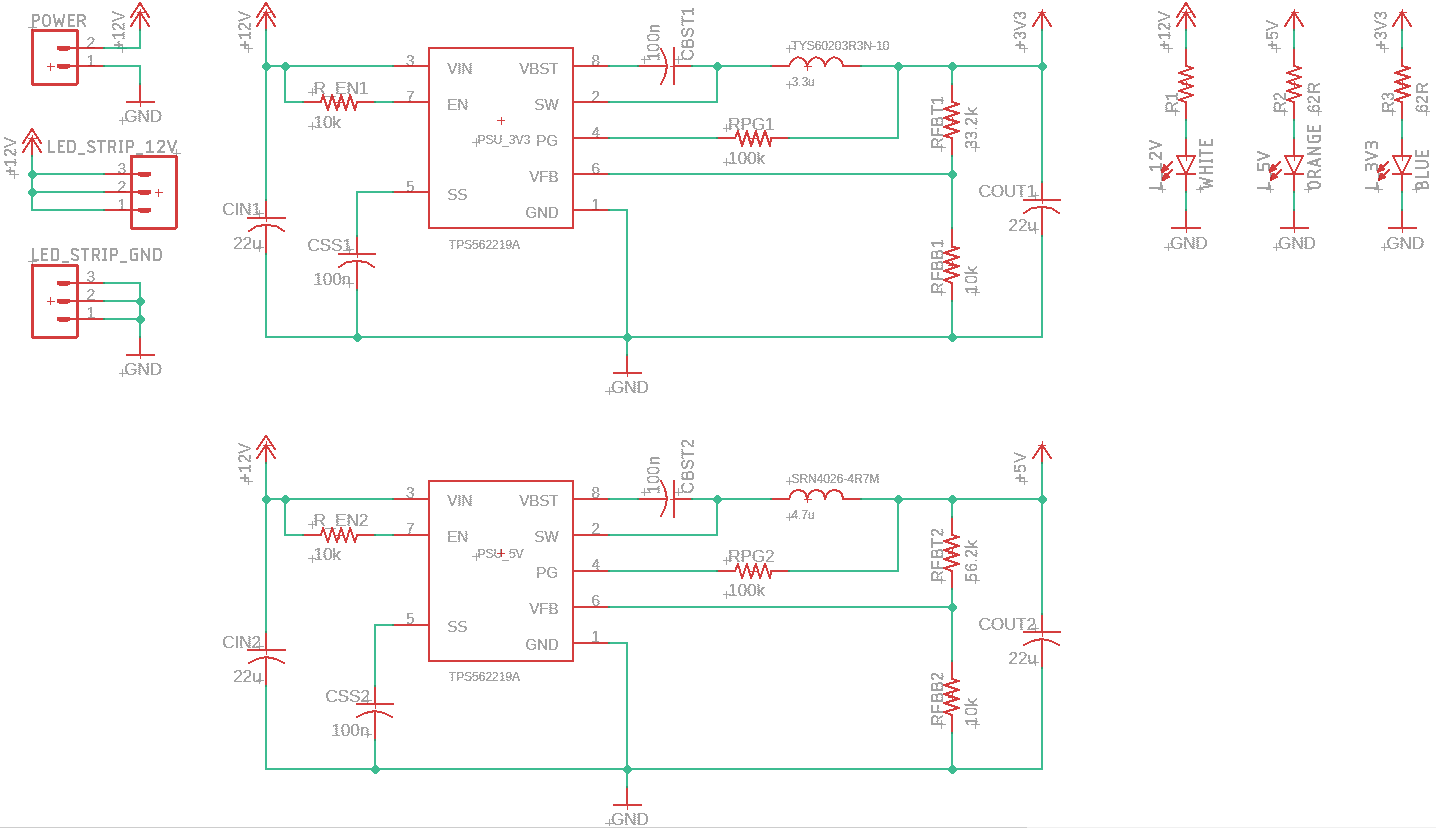
\includegraphics[width=20cm, angle=90]{resources/pcb_res/big_schematic01.png}
            \caption{}
            \label{fig:android_things}
        \end{figure}

        \begin{figure}[h!]
            \centering
            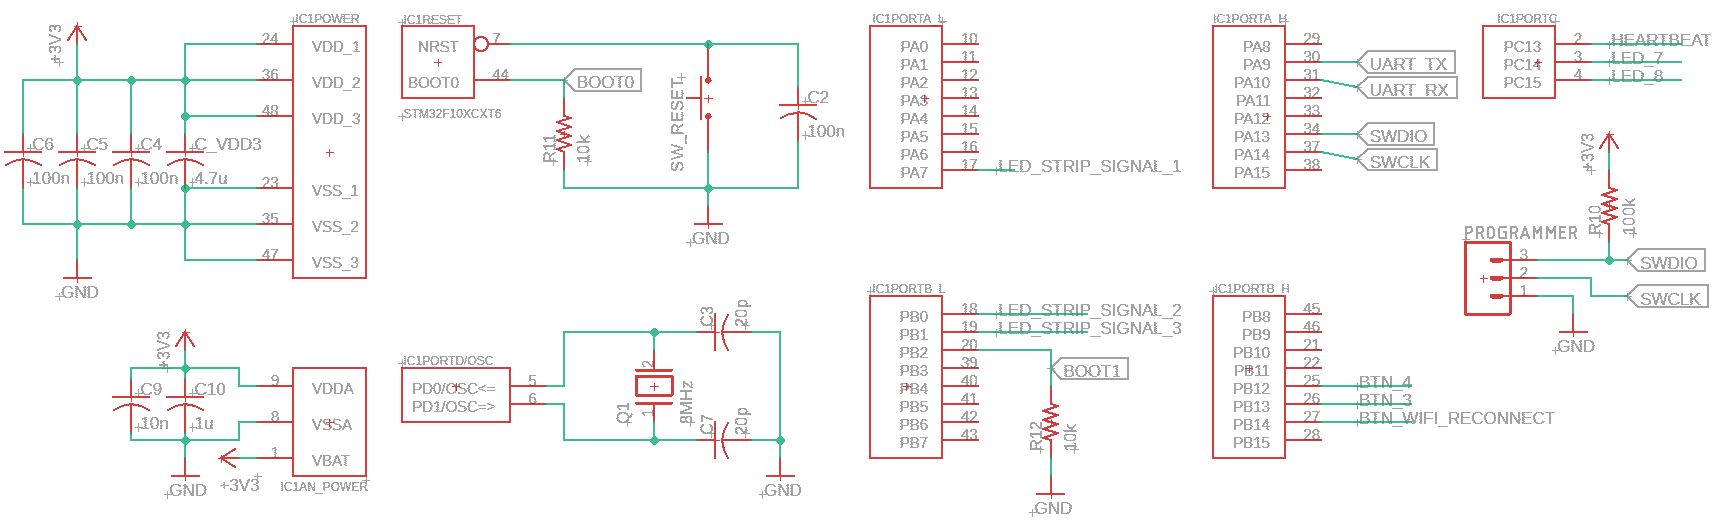
\includegraphics[width=23cm, angle=90]{resources/pcb_res/big_schematic02.png}
            \caption{}
            \label{fig:android_things}
        \end{figure}
        
        \begin{figure}[h!]
            \centering
            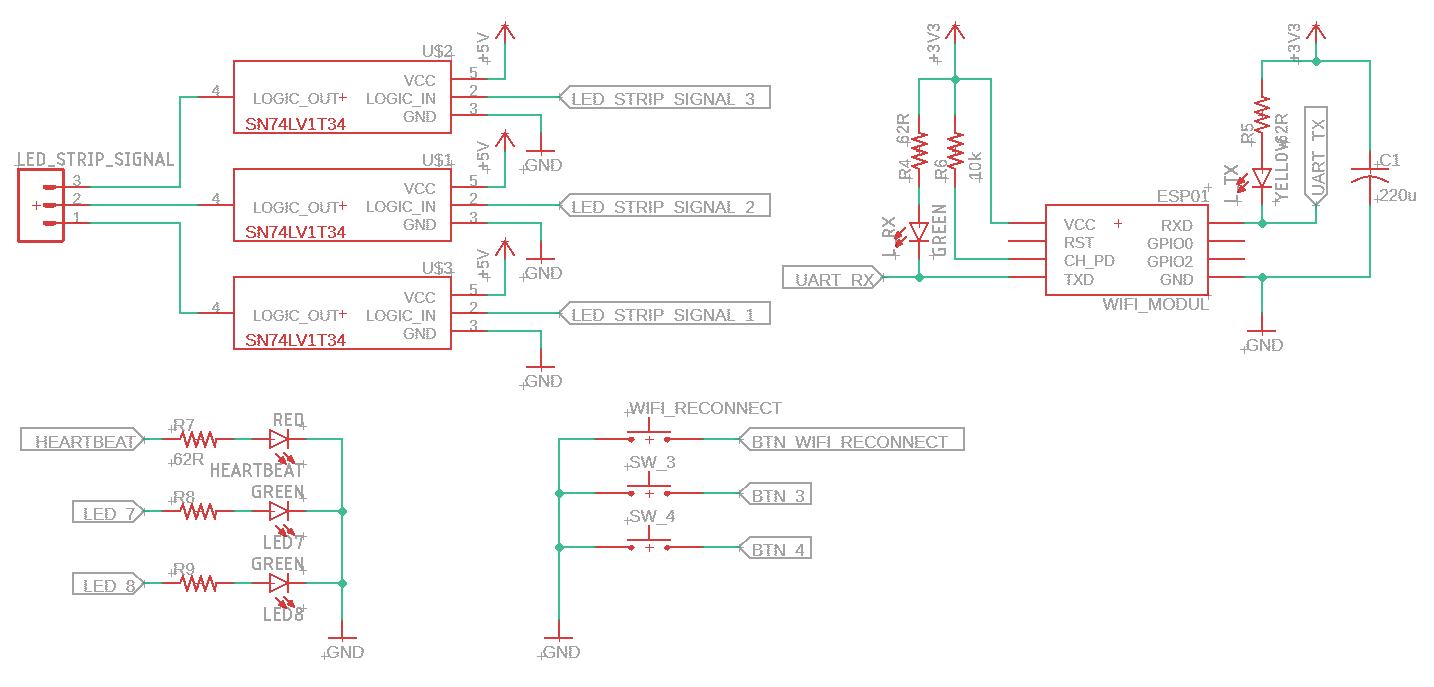
\includegraphics[width=20cm, angle=90]{resources/pcb_res/big_schematic03.png}
            \caption{}
            \label{fig:android_things}
        \end{figure}
        
\end{document}